\chapter{Toolset for Analyzing Application-aware Dynamic Interconnects}

\hypertarget{introduction}{%
\section{Introduction}\label{introduction}}

Inter-node communication performance of High Performance Computing (HPC)
clusters heavily affects the total performance of
communication-intensive applications. Communication-intensive
applications require low-latency and high-bandwidth communication
between computing nodes to fully exploit the computational power and
parallelism of the computing nodes. High performance networks that
provide such low-latency and high-bandwidth communication between
computing nodes of a cluster are often referred to as
\emph{interconnects}. Message Passing Interface
(MPI)~\autocites{MessagePassingInterfaceForum2015}{Gropp2014} is a
commonly used inter-process communication library to describe
communication on HPC clusters.

In this paper, interconnects are roughly classified into \emph{static
interconnects} and \emph{dynamic interconnects}. In the former category,
it is assumed that packet flow is controlled solely based on its source
and/or destination. A well-known exemplifier is
InfiniBand~\autocite{InfiniBand2015}, where forwarding tables of
switches are populated with pre-computed forwarding rules in advance of
the execution of applications. In contrast, in the latter category, it
is assumed that packet flow is dynamically controlled to mitigate load
imbalance and improve utilization of the interconnect.

Nowadays, the majority of HPC clusters employ the former static
interconnects because of the low implementation cost. Since static
interconnects are controlled without taking the communication patterns
of individual applications into account, they are usually designed to be
able to accommodate the worst-case traffic demand to achieve good
performance for a variety of applications, each of which has a different
communication pattern. Interconnect designers have respected criteria
such as full bisection bandwidth and nonblocking networks.

The continuously growing demand for computing power from academia and
industry has inevitably forced HPC clusters to scale out more and more.
As a result of the growing number of computing nodes, interconnects are
becoming increasingly large-scale and complex. This technical trend is
making static and over-provisioned interconnects cost-ineffective and
difficult to build.

Based on this background and these trends, we study the feasibility and
applicability of programming dynamic interconnect within
HPC~\autocite{Date2016}. In particular, \emph{SDN-enhanced
MPI}~\autocites{Takahashi2014}{Dashdavaa2013}, a framework that
incorporates the dynamic network controllability of Software-Defined
Networking (SDN)~\autocite{sdn} into MPI, has been researched based on
the idea that dynamically optimizing the packet flow in the interconnect
according to the communication patterns of applications can increase the
utilization of the interconnect and improve application performance. The
goal of SDN-enhanced MPI is to accelerate individual MPI functions by
dynamically optimizing the packet flow in the interconnect. Several MPI
functions have been successfully accelerated in our previous works so
far. One of the core challenges in the research of SDN-enhanced MPI is
to develop algorithms to control the packet flow in the interconnect
depending on the MPI function called by the application.

More generally, algorithms for efficiently controlling the packet flow
in the interconnect depending on the communication patterns of
applications is essential towards realizing a dynamic and
application-aware interconnect. In order to develop a generic algorithm
that achieves good performance on a variety of environments, the
algorithm must be investigated and evaluated by targeting different
applications and interconnects. However, utilizing physical clusters to
analyze the performance characteristics of the interconnect is
restricted in the following points. First, the execution time of
real-world HPC applications typically ranges from hours up to days,
sometimes even months. Second, large-scale deployments of dynamic
interconnects that allow execution of highly parallel applications have
not yet been seen because research and development of dynamic
interconnects are still at their early stage. Third, network hardware
such as switches may not support measuring traffic in the interconnect
with enough high frequency and precision to obtain meaningful insights.

To accelerate the research and development of application-aware dynamic
interconnects that control packet flow in response to the communication
patterns of applications, an interconnect simulator that allows users to
conduct systematic investigation of clusters with diverse topologies and
parameters is vitally demanded. A wide spectrum of interconnect
simulators have been developed with different focus and purpose until
today. However, existing simulators mostly focused on static
interconnects and little research has been done to simulate dynamic and
application-aware interconnects.

This paper describes the design and implementation of PFAnalyzer, a
toolset for analyzing application-aware dynamic interconnects.
PFAnalyzer consists of two components: PFSim and PFProf. PFSim is an
interconnect simulator specialized for application-aware dynamic
interconnects. PFSim takes a set of communication patterns of
applications and a cluster configuration as its input and then simulates
the traffic on each link of the interconnect. PFProf is a custom
profiler to extract communication patterns from applications for use in
conjunction with PFSim.

The contributions of this paper are summarized as follows:

\begin{itemize}
\item
  A lightweight interconnect simulator for simulating dynamic and
  application-aware interconnects is proposed.
\item
  A custom profiler for extracting communication patterns from
  applications is presented.
\item
  Simulation results for NAS CG benchmark and MILC on a fat-tree
  interconnect are presented.
\end{itemize}

The rest of this paper is organized as follows.
Section~\ref{research-objective} examines the requirements of an
interconnect simulator for dynamic and application-aware interconnects.
Section~\ref{related-work} reviews related work. Section~\ref{proposal}
describes the design and implementation of PFAnalyzer.
Section~\ref{evaluation} presents the simulation results for NAS CG
benchmark and MILC obtained with our proposed simulator. Furthermore,
results of a verification experiment on a physical cluster are shown.
Section\\
\ref{conclusion} concludes this paper and outlines our future work.

\hypertarget{research-objective}{%
\section{Research Objective}\label{research-objective}}

In this paper, we aim to realize an interconnect simulator specialized
for application-aware dynamic interconnects to facilitate the research
and development of application-aware dynamic interconnects. Most
interconnect simulators proposed in the previous
research~\autocites{Schneider2009}{Tikir2009}{Hoefler2010}{Jo2015} are
designed to study the behavior of static interconnects. Therefore,
packet flow is controlled based on static routing algorithms in these
simulators.

However, packet flow needs to be dynamically controlled based on the
communication patterns of applications for simulating application-aware
dynamic interconnects. Based on this necessity, the requirements for our
simulator are described as follows:

\begin{itemize}
\item
  \emph{Support for application-aware dynamic routing}: The simulator
  should allow users to implement dynamic routing algorithms to mitigate
  load imbalance and improve utilization of the interconnect. In
  addition, the routing algorithms should be supplied with the
  communication patterns of applications and packet flow in the
  interconnect to make effective routing decisions.
\item
  \emph{Support for communication patterns of real-world applications}:
  Communication patterns of real-world HPC applications should be fed
  into the simulator to reproduce the characteristics of communication
  generated by real-world applications. To simulate the packet flow in
  the interconnect when an application is being executed, the simulator
  needs to predict the volume of point-to-point communication exchanged
  between computing nodes. In the actual computing scene, the traffic
  among computing nodes is generated by the processes executed on the
  computing nodes. Thus, some means and mechanisms to analyze the
  traffic volume of point-to-point communication exchanged between the
  processes from applications is essential. In this paper, applications
  that leverage MPI for inter-process communication are targeted.
\item
  \emph{Support for diverse cluster configurations}: The distribution of
  packet flow in the interconnect is determined by not only the routing
  algorithm but also the topology of the interconnect. In addition, job
  scheduling, node selection and process placement algorithms need to be
  considered. These parameters should be easily reconfigurable to allow
  users to perform a systematic investigation of diverse clusters.
\end{itemize}

Furthermore, the simulator should be designed to be lightweight and fast
to carry out a large number of simulations with different parameters in
a reasonable amount of time. If necessary, appropriate approximation
should be introduced to improve simulation performance.

\hypertarget{related-work}{%
\section{Related Work}\label{related-work}}

Several interconnect simulators have been proposed in past research.
PSINS~\autocite{Tikir2009} is a trace-driven simulator for HPC
applications. Traces obtained from applications are used to predict the
performance of applications on a variety of HPC clusters with different
configurations. LogGOPSim~\autocite{Hoefler2010} simulates the execution
of MPI applications based on the LogGOP network model. Both simple
synthetic communication patterns and communication patterns converted
from traces of MPI applications can be fed into the simulator. A
limitation of LogGOPSim is that the interconnect is assumed to have full
bisection bandwidth and congestion is not simulated. These two
simulators can provide accurate performance predictions owing to their
per-message simulation capability. However, the topology and the routing
algorithm of interconnects are abstracted in the network models of PSINS
and LogGOPSim. Therefore, these simulators cannot be used for predicting
and comparing the performance of different topologies or routing
algorithms. In contrast, the simulator targeted in this paper allows
users to compare the performance characteristic of different topologies
and routing algorithms.

ORCS~\autocite{Schneider2009} simulates the traffic load of each link in
the interconnect for a given topology, communication pattern and routing
algorithm. The simulated traffic load of links can be summarized into
various performance metrics and used for further analysis. A limitation
of ORCS is that only pre-defined communication patterns can be used as
its input. Moreover, ORCS assumes static routing as in InfiniBand. On
the contrary, our simulator can handle dynamic routing algorithms that
use communication patterns of applications and interconnect usage to
make routing decisions.

In \autocite{Jo2015}, simulations are carried out to examine the
performance characteristics of an SDN-based multipath routing algorithm
for data center networks. A simulator is developed based on MiniSSF to
simulate the throughput and delay of a packet flow under diverse
settings. However, communication patterns are randomly generated and not
based on real-world applications. Our proposed simulator is designed to
accept arbitrary communication patterns obtained from real-world
applications using our custom profiler.

\(\mathit{INAM}^2\) \autocite{Subramoni2016} is a comprehensive tool to
monitor and analyze network activities in an InfiniBand network. The
tight integration with the job scheduler and a co-designed MPI library
allows \(\mathit{INAM}^2\) to associate network activities with jobs and
MPI processes. For instance, it can identify hot spots in the
interconnect and inspect which node, job, and process is causing the
congestion. Although \(\mathit{INAM}^2\) is a useful tool for system
administrators to diagnose the performance issues of interconnects, it
is not suitable for studying diverse interconnects since it only
supports physical clusters.

\hypertarget{proposal}{%
\section{Proposal}\label{proposal}}

We propose \emph{PFAnalyzer}, a toolset for analyzing the performance
characteristics of application-aware dynamic interconnects. PFAnalyzer
is composed of \emph{PFProf}, a profiler to extract communication
patterns from applications, and \emph{PFSim}, a simulator capable of
simulating application-aware dynamic interconnects.

\hypertarget{representation-of-a-communication-pattern}{%
\subsection{Representation of a Communication
Pattern}\label{representation-of-a-communication-pattern}}

In this paper, we represent the communication pattern of an application
using the traffic matrix of the application. For an application composed
of \(n\) processes, its traffic matrix is defined as a \(n \times n\)
square matrix \(T\) of which element \(T_{ij}\) is equal to the volume
of traffic sent from rank \(i\) to rank \(j\). Here, we approximate the
volume of traffic between processes as constant during the execution of
a job. The traffic volume between a process pair is assumed to be the
total bytes transferred divided by the duration of the application.

This approximation is introduced to simplify and speed up the
simulation. The idea behind this approximation is based on the fact that
many HPC applications (\emph{e.g.} partial differential equation
solvers) show an iterative nature. These applications spend most of
their execution time inside a repetitive loop and thus their
communication patterns do not significantly change over time. Therefore,
the traffic matrix can be a good representation of the communication
characteristics of an iterative application despite the loss of temporal
order. In the future, we plan to apply trace
segmentation~\autocite{Alawneh2016} techniques on the communication
trace. This technique will segment a trace into multiple communication
phases, which could then be simulated individually to further improve
the accuracy of simulation for applications with significantly
time-varying communication patterns.

\hypertarget{pfprof-mpi-profiler}{%
\subsection{PFProf (MPI Profiler)}\label{pfprof-mpi-profiler}}

Initially, we tried to reuse existing MPI performance analysis tools
such as \mbox{Score-P}~\autocite{Knupfer2012},
Vampir~\autocite{Knupfer2008} and Tau~\autocite{Shende2006} to collect
the traffic matrices from MPI applications. However, these tools capture
only a subset of the communication pattern when profiling an application
that uses collective communication functions (\emph{e.g.} MPI\_Bcast,
MPI\_Allreduce and MPI\_Reduce).

The reason can be explained as follows. Existing MPI profilers replace
the standard MPI functions provided by MPI libraries with instrumented
functions by utilizing the MPI Profiling Interface (PMPI). An advantage
of this approach is that it works regardless of a specific MPI
implementation. However, this approach fails to capture the internal
information of the MPI library. Meanwhile, collective communication
functions are internally implemented as a combination of point-to-point
communication in MPI implementations. These underlying point-to-point
communication functions are hidden from PMPI-based profilers and
excluded from the communication patterns emitted by profilers.

To accurately capture the underlying point-to-point communication of
collective communication, we have developed a profiler by utilizing the
MPI Performance Examination and Revealing Unexposed State Extension
(PERUSE)~\autocite{Jones2006}. PERUSE was designed to provide internal
information of the MPI implementation that were not exposed through PMPI
to applications and performance analysis tools. By using PERUSE,
application or performance analysis tools register callback functions
for each event of interest. After that, the registered callback function
is called each time when the associated event occurs.

Figure~\ref{fig:profiler-block} illustrates how PFProf, MPI library and
MPI application interact with each other. PFProf hooks MPI\_Init and
MPI\_Finalize to perform initialization and finalization. During the
initialization, PFProf subscribes to two PERUSE events:
\lstinline!PERUSE\_COMM\_REQ\_XFER\_BEGIN! and
\lstinline!PERUSE\_COMM\_REQ\_XFER\_END!. These events are
emitted each time a transfer of a message begins and ends, respectively.
Profiling results are written out as a JSON file during the
finalization. During the execution of an application, the total number
of bytes transferred from a process to another is aggregated to compute
the traffic matrix.

\begin{figure}[htbp]
    \centering
    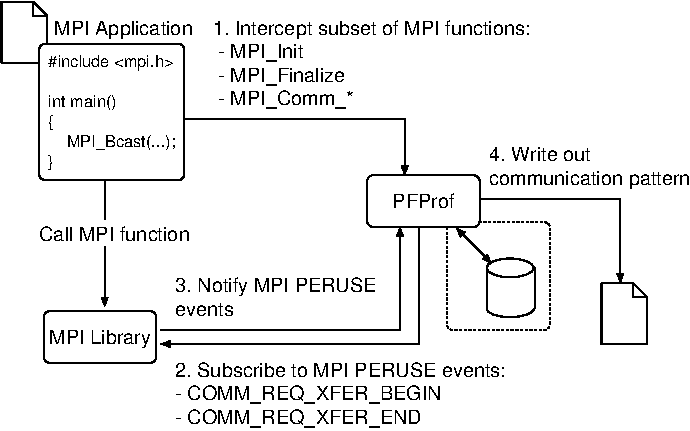
\includegraphics[scale=.9]{tracer_block}
    \caption{Block Diagram of PFProf}
    \label{fig:profiler-block}
\end{figure}

Furthermore, PFProf hooks several MPI functions to create and destroy
communicators to maintain a mapping between global ranks (rank number
within \lstinline!MPI\_COMM\_WORLD!) and local ranks (rank
number within communicators created by users). This mapping is necessary
because PERUSE events are reported with local ranks, while profiling
results should be described with global ranks for the ease of analysis.

PFProf is provided in the form of a shared library, which can be
integrated into applications either when building the application or
running the application. The preferred way is to use run-time
integration, because it requires neither recompilation nor relinking of
the application. The \lstinline!LD\_PRELOAD! environment
variable is used to load the shared library before the execution of the
application.

A visualization of a traffic matrix obtained from running MILC with 128
processes is shown in Fig.~\ref{fig:traffic-matrix}. This visualization
clearly reveals the spatial locality and sparsity of the communication
pattern.

\begin{figure}[htbp]
    \centering
    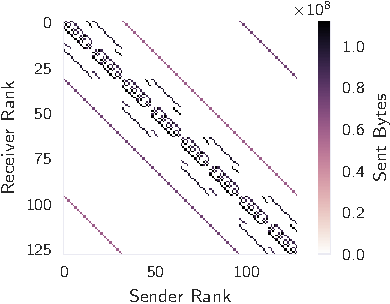
\includegraphics{traffic_matrix}
    \caption{Traffic Matrix for MILC}
    \label{fig:traffic-matrix}
\end{figure}

\hypertarget{pfsim-interconnect-simulator}{%
\subsection{PFSim (Interconnect
Simulator)}\label{pfsim-interconnect-simulator}}

PFSim uses a set of communication patterns of applications and a cluster
configuration as its input and then simulates the packet flow generated
by the applications. The packet flow is aggregated per link to compute
the traffic load of each link. The simulated traffic load of links can
be summarized into statistics for quantitative analysis or visualized.
Using these outputs from PFSim, users can locate hot-spots and assess
load imbalance in the interconnect. These insights on the interconnect
can be useful for designing better algorithms for controlling the packet
flow in application-aware dynamic interconnects.

PFSim is based on a discrete-event simulation model. Under this model,
each event holds an attribute indicating when it will occur. Events are
stored in a priority queue in an increasing manner by the time they
occur. There are different type of events representing a change of state
in the simulator such as: a job arrived, a job started, a job finished,
\emph{etc}. At the beginning of the main loop, the earliest occurring
event is popped from the event queue. Then, based on the type of the
event, the corresponding event handler is called. An event handler may
schedule new events. This loop is repeated until the event queue is
empty.

Figure~\ref{fig:simulator-block} illustrates how PFSim works. The
simulation scenario file defines various configurations for a simulation
run. This file defines the cluster configuration to use and the set of
jobs. Moreover, algorithms that control the execution and communication
of jobs are specified as shown in Table~\ref{tbl:simulator-algorithm}.
An example of a simulation scenario file is shown in
Listing~\ref{lst:simulation-scenario}. The cluster configuration file
defines the topology of the interconnect, the capacity of links, and the
number of processing elements for each computing node. This file is
described in GraphML~\autocite{Brandes2013}, an XML-based markup
language for graphs. Popular graph visualization tools such as Cytoscape
and Gephi can be used to view and edit GraphML files. Communication
pattern files are obtained from applications using PFProf described in
the previous section \ref{pfprof-mpi-profiler}.

\begin{figure}[htbp]
    \centering
    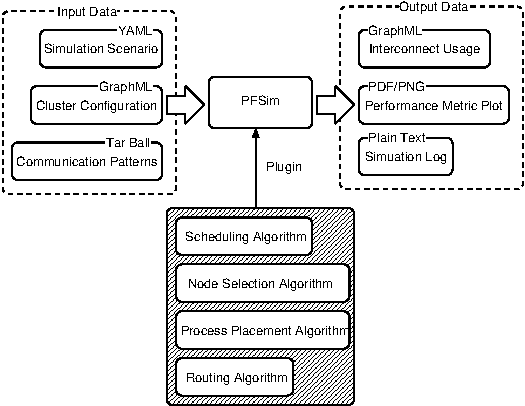
\includegraphics[scale=.9]{simulator_block}
    \caption{Block Diagram of PFSim}
    \label{fig:simulator-block}
\end{figure}

Each configuration value can be a list of values. In that case, the
simulation is executed multiple times, each time with a different
combination of configuration values until all combinations are
completed.

\begin{table}[htbp]
    \centering
    \normalsize
    \caption{List of Configurable Algorithms}
    \label{tbl:simulator-algorithm}
    \begin{tabularx}{\linewidth}{lX}
        \hline
        Algorithm         & Description                                                 \\
        \hline \hline
        Job Scheduling    & Selects the job to execute from the job queue.
                            (\emph{e.g.} FCFS, Backfill)                                \\ \hline
        Node Selection    & Selects which computing nodes to assign for a job.
                            (\emph{e.g.} Linear, Random, Topology-aware algorithms)     \\ \hline
        Process Placement & Determines on which computing node to place a process.
                            (\emph{e.g.} Block, Cyclic, Application-aware algorithms)   \\ \hline
        Routing           & Computes a route between a pair of processes.
                            (\emph{e.g.} D-mod-K, S-mod-K, Random, Dynamic algorithms)  \\ \hline
    \end{tabularx}
\end{table}

PFSim can create a snapshot of the traffic distribution in the
interconnect at an arbitrary time and output is as a GraphML file. By
visualizing the acquired GraphML using the aforementioned graph
visualization tools, users can intuitively locate bottleneck links and
load imbalance. Furthermore, the traffic load of links can be summarized
into statistics such as maximum, minimum, average, variance and plotted
as graphs.

\begin{lstlisting}[caption={Example of a Simulation Scenario}, label={lst:simulation-scenario}, linewidth={\columnwidth}]
topology: topologies/milk.graphml
output: output/milk-cg-dmodk
algorithms:
  scheduler:
    - pfsim.scheduler.FCFSScheduler
  node_selector:
    - pfsim.node_selector.LinearNodeSelector
    - pfsim.node_selector.RandomNodeSelector
  process_mapper:
    - pfsim.process_mapper.LinearProcessMapper
    - pfsim.process_mapper.CyclicProcessMapper
  router:
    - pfsim.router.DmodKRouter
    - pfsim.router.GreedyRouter
    - pfsim.router.GreedyRouter2
jobs:
  - submit:
      distribution: pfsim.math.ExponentialDistribution
      params:
        lambd: 0.1
    trace: traces/cg-c-128.tar.gz
...
\end{lstlisting}

\begin{figure}[h]
    \centering
    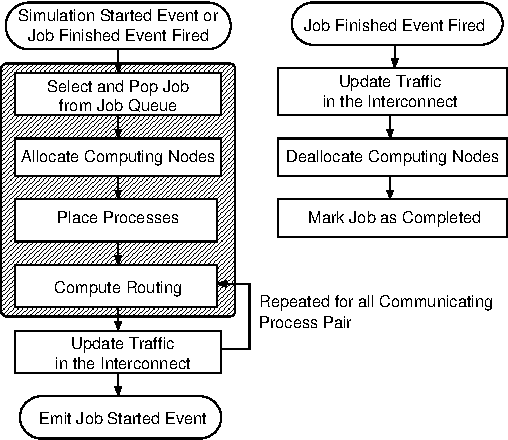
\includegraphics{simulator_flowchart}
    \caption{Life Cycle of a Simulated Job}
    \label{fig:simulator-flowchart}
\end{figure}

Figure~\ref{fig:simulator-flowchart} illustrates the life cycle of a
simulated job. On arrival of a new job, the job is initially enqueued to
the job queue. As soon as there are enough unallocated computing nodes
to execute a job, the scheduling algorithm determines the job to be
executed next and pops it from the job queue. Subsequently, the node
selection algorithm picks a set of computing nodes that can satisfy the
requested number of processes by the job. Then, the process placement
algorithm determines on which computing node to run each process of the
job. After the process placement is completed, the routing algorithm
computes and allocates routes for all communicating pairs of processes.
To allow users to implement application-aware dynamic routings,
additional information is supplied to the routing algorithm in addition
to the source/destination process pair. The information includes process
placement, communication patterns and interconnect usage. For each
allocated route, the traffic on the link contained in the route is
increased. After all routes are computed, PFSim waits until the job has
finished. Then, the traffic for each link that was utilized by the job
is decreased. Finally, computing nodes are deallocated and the job is
marked as completed.

\hypertarget{evaluation}{%
\section{Evaluation}\label{evaluation}}

In this section, we first simulate the traffic load of a fat-tree
interconnect when using static interconnect control and dynamic
interconnect control. Subsequently, benchmark results obtained from a
physical cluster are used to investigate the impact of traffic load on
the application performance. Lastly, we assess the overhead incurred by
our profiler.

\hypertarget{simulation-results}{%
\subsection{Simulation Results}\label{simulation-results}}

In this experiment, communication-intensive MPI applications were
executed on our simulator. The maximum traffic load observed on links
composing the interconnect was compared in both cases of static
interconnect control and dynamic interconnect control. The maximum
traffic load observed on the links was used as an indicator of the
communication performance of an application. In most cases, a hot spot
link can slow down the whole application, because when collective
communication or synchronization is performed by an application, every
process needs to wait until the slow communication crossing the hot spot
link completes. Therefore, mitigating the traffic load on the hot spot
link could improve the performance of the application.

The simulated cluster was modeled after a physical cluster installed at
our institution. It was composed of 20 computing nodes, each equipped
with 8 cores. Computing nodes were interconnected with a fat-tree
topology as illustrated in Fig.~\ref{fig:cluster-config}.

\begin{figure}[htbp]
    \centering
    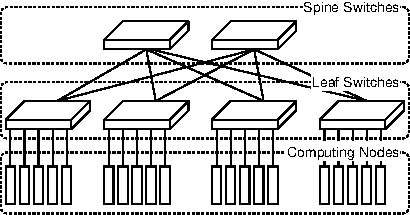
\includegraphics{cluster_config}
    \caption{Simulated Cluster with Fat-Tree Interconnect}
    \label{fig:cluster-config}
\end{figure}

Two applications were selected as representatives of
communication-intensive applications. The first one is the CG benchmark
from the NAS Parallel Benchmark Suite~\autocite{Bailey1991}. The CG
benchmark estimates the largest eigenvalue of a sparse matrix using the
inverse power method. Internally it uses the conjugate gradient method,
which frequently appears in irregular mesh applications. The second
application (\lstinline!ks\_imp\_dyn!) is from MIMD
Lattice Computation (MILC)~\autocite{milc}, a collection of applications
used to study Quantum Chromodynamics (QCD). We used the input dataset
provided by NERSC as a part of the NERSC MILC benchmark. These two
applications were executed with 128 MPI processes. Thread parallelism
was not put in use (\emph{i.e.} a flat MPI model was adopted).

To analyze the effect of dynamic interconnect control, simulations were
carried out either using static routing or dynamic routing. Furthermore,
in order to investigate the impact of node selection and process
placement to the traffic load, the node selection algorithm and process
placement algorithm were also changed. As a result, exhaustive
combinations of two node selection algorithms, two process placement
algorithms and two routing algorithms were investigated with the
scheduling algorithm fixed. Below are the descriptions of the algorithms
used in this experiment:

\begin{itemize}
\item
  Scheduling: A simple \emph{First-Come First-Served (FCFS)} scheduling
  without backfilling was adopted.
\item
  Node Selection: Either \emph{linear} or \emph{random} node selection
  was adopted. Linear node selection assumes that computing nodes are
  lined up in a one-dimensional array and minimizes the fragmentation of
  allocation. This is essentially the same as the default node selection
  policy of Slurm. Random node selection randomly selects computing
  nodes. This algorithm simulates a situation where the allocation of
  computing nodes is highly fragmented.
\item
  Process Placement: Either \emph{block} or \emph{cyclic} process
  placement was adopted. Block process placement assigns rank \(i\) to
  the \(\lfloor i / c \rfloor\)-th computing node where \(c\) represents
  the number of cores per node. Cyclic process placement assigns rank
  \(i\) to the \((i \bmod n)\)-th computing node where \(n\) denotes the
  number of computing nodes.
\item
  Routing: Either \emph{D-mod-K} routing or a \emph{dynamic} routing was
  adopted. \mbox{Destination-modulo-K} (\mbox{D-mod-K}) routing is a
  popular static load balancing routing algorithm that distributes
  packet flow over multiple paths based on the destination address of
  the packet. The dynamic routing algorithm implemented here computes
  and allocates routes from the heaviest communicating process pair. A
  route is computed to minimize the traffic of the maximum-traffic link
  in the path.
\end{itemize}

Under this condition, we measured and compared the maximum traffic load
observed on links through the simulation.
Figure~\ref{fig:nas-cg-multi-congestion} shows the simulation results in
the NAS CG benchmark. In this graph, red bars represent the results of
\mbox{D-mod-K} routing while blue bars represent the results of dynamic
routing. The vertical axis represents the simulated maximum traffic load
normalized by the maximum traffic load when linear node selection, block
process placement and \mbox{D-mod-K} routing is adopted.

What stands out in Fig.~\ref{fig:nas-cg-multi-congestion} is that
dynamic routing consistently achieves lower traffic load compared to
static \mbox{D-mod-K} routing. The reduction of traffic load was largest
when linear node selection and block process placement were adopted.
Under this combination of node selection and the process placement
algorithm, dynamic routing slashed the maximum traffic load by 50\%
compared to \mbox{D-mod-K} routing. In addition, the graph reveals that
cyclic process placement always increased maximum traffic load compared
to block process placement because neighboring ranks were placed on
different computing nodes despite the locality of the communication
pattern.

\begin{figure}[htbp]
    \centering
    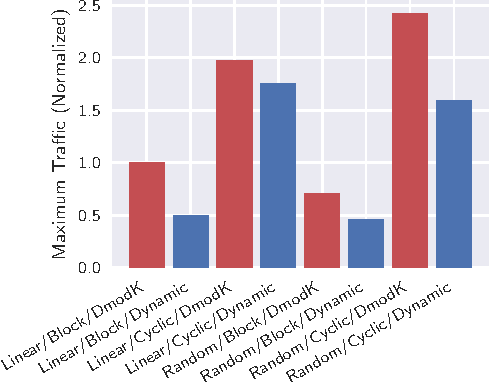
\includegraphics[scale=.9]{nas_cg_multi_congestion}
    \caption{Comparison of Maximum Traffic (NAS CG)}
    \label{fig:nas-cg-multi-congestion}
\end{figure}

\begin{figure}[htbp]
    \centering
    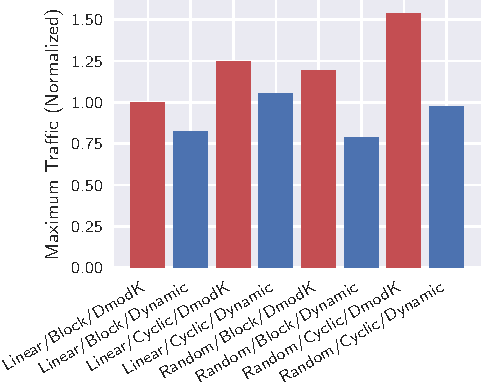
\includegraphics[scale=.9]{nersc_milc_multi_congestion}
    \caption{Comparison of Maximum Traffic (MILC)}
    \label{fig:nersc-milc-multi-congestion}
\end{figure}

Figure~\ref{fig:nersc-milc-multi-congestion} shows the result in the
case of MILC\@. The graph reveals that dynamic routing outperforms
\mbox{D-mod-K} routing. In this case, the reduction of the link load was
largest when random node selection and cyclic process placement was
adopted. When using linear node selection and block process placement,
reduction of the maximum link load was 18\%.

\hypertarget{benchmark-results}{%
\subsection{Benchmark Results}\label{benchmark-results}}

To investigate the impact of traffic load on the application performance
of an actual environment, we reproduced the configuration described in
the previous section \ref{simulation-results} on a physical cluster and
then measured the execution time of each benchmark. This cluster was
equipped with switches that support OpenFlow, which is a de facto
standard implementation of SDN\@. The routing algorithms were implemented
based on OpenFlow. In this experiment, linear node selection and block
process placement was adopted. The average execution time of 10 runs was
compared when using \mbox{D-mod-K} routing and dynamic routing.
Figure~\ref{fig:nas-cg-time} shows the comparison for the NAS CG
benchmark. The graph indicates that the use of dynamic routing reduced
the execution time of the benchmark to 23\%.
Figure~\ref{fig:nersc-milc-time} shows the result for MILC\@. In this
case, approximately 8\% was reduced in execution time.

These results suggest that application performance is actually improved
by alleviating the traffic load on the hot spot link. This suggestion
implies that researchers of dynamic interconnects can take advantage of
our toolset to simulate different packet flow controlling algorithms and
assess their performance improvement effect on real-world applications
by using indicators such as maximum traffic load.

\begin{figure}[htbp]
    \begin{subfigure}[t]{.47\linewidth}
        \centering
        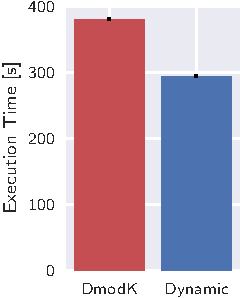
\includegraphics[scale=.9]{nas_cg_execution_time}
        \caption{NAS CG}
        \label{fig:nas-cg-time}
    \end{subfigure}%
    \begin{subfigure}[t]{.47\linewidth}
        \centering
        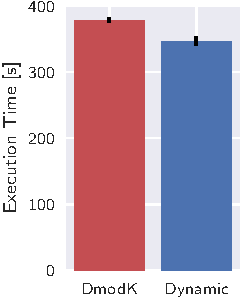
\includegraphics[scale=.9]{nersc_milc_execution_time}
        \caption{MILC}
        \label{fig:nersc-milc-time}
    \end{subfigure}
    \caption{Comparison of Execution Time}
    \label{fig:single-job-time}
\end{figure}

\hypertarget{profiling-overhead}{%
\subsection{Profiling Overhead}\label{profiling-overhead}}

In this experiment, the performance of point-to-point communication
between two processes with and without PFProf were compared to inspect
the overhead incurred by the profiler. OSU Micro
Benchmark~\autocite{omb} was used to measure the throughput and latency
of point-to-point communication between two processes for varying
message sizes. The comparison of throughput is shown in
Fig.~\ref{fig:bandwidth-overhead}. For messages larger than 1KB, the
overhead was ignorable. For messages smaller than 1KB, up to 30\% of
overhead was incurred. Benchmark results for latency, as shown in
Fig.~\ref{fig:latency-overhead}, suggest that there is almost no
overhead for latency.

\begin{figure}[htbp]
    \centering
    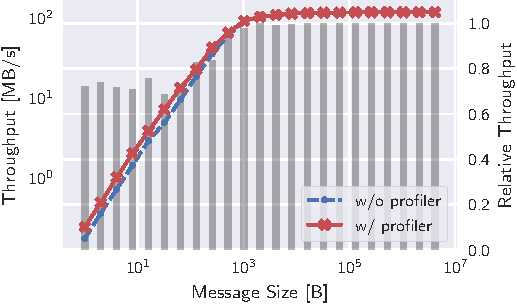
\includegraphics[scale=.9]{bandwidth_overhead}
    \caption{Throughput of MPI\_Send/Recv Between Two Nodes}
    \label{fig:bandwidth-overhead}
\end{figure}

\begin{figure}[htbp]
    \centering
    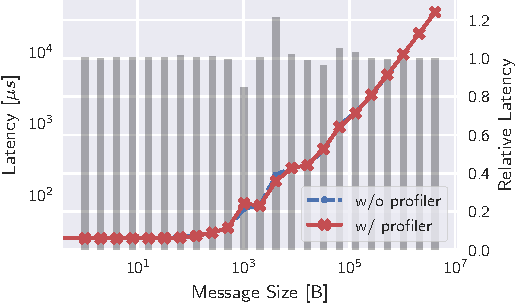
\includegraphics[scale=.9]{latency_overhead}
    \caption{Latency of MPI\_Send/Recv Between Two Nodes}
    \label{fig:latency-overhead}
\end{figure}

\hypertarget{conclusion}{%
\section{Conclusion}\label{conclusion}}

This paper described the design and implementation of PFAnalyzer, a
toolset for analyzing the performance characteristics of
application-aware dynamic interconnects. PFAnalyzer is composed of
PFProf, a profiler to extract communication patterns from applications,
and PFSim, a simulator capable of simulating application-aware dynamic
interconnects. PFSim takes a set of communication patterns of
applications and a cluster configuration as its input and then simulates
the traffic on each link of the interconnect. Our evaluation shows how
dynamically controlling the interconnects can reduce congestion and
potentially improve the performance of applications.

Further work is necessary to investigate the performance characteristics
of dynamic interconnects on large-scale and highly parallel clusters.
Moreover, we plan to implement application-aware node selection and
process placement algorithms on PFSim. The impact of such
application-aware algorithms on the performance of dynamic interconnects
should be evaluated.
